\documentclass{exam}
\usepackage[utf8]{inputenc}
\usepackage{lmodern}
\usepackage{microtype}

% \usepackage[parfill]{parskip}
\usepackage[dvipsnames]{xcolor}
\usepackage{amsmath}
\usepackage{amsfonts}
\usepackage{amsthm}
\usepackage{siunitx}
\DeclareSIUnit\year{yr}
\DeclareSIUnit\foot{ft}
\DeclareSIUnit\litre{\liter}

\usepackage{skull}

\usepackage{pgfplots}
\usepgfplotslibrary{polar}
\pgfplotsset{compat=1.11}
\usepgfplotslibrary{statistics}
\usepackage{graphicx}
\usepackage{sidecap}
\sidecaptionvpos{figure}{c}
\usepackage{float}
\usepackage{gensymb}
\usepackage{tkz-euclide}
\usetkzobj{all}
\usepackage{commath}
\usepackage{hyperref}
\usepackage{enumitem}
\usepackage{wasysym}
\usepackage{multicol}
\usepackage{mathtools}
\usepackage{tcolorbox}
\usepackage{tabularx}
\usepackage[version=4]{mhchem}
\usepackage{changepage}
\usepackage{listings}
\lstset{basicstyle=\ttfamily\linespread{0.8}\small}

\renewcommand*{\thefootnote}{\fnsymbol{footnote}}

\newtheorem*{thm}{Theorem}
\newtheorem*{iden}{Identity}
\newtheorem*{lemma}{Lemma}
\newtheorem{obs}{Observation}
\theoremstyle{definition}
\newtheorem*{defn}{Definition}
\newtheorem*{ex}{Example}
\newtheorem{con}{Construction}
\newtheorem*{alg}{Algorithm}

\newtheoremstyle{break}
  {\topsep}{\topsep}%
  {\itshape}{}%
  {\bfseries}{}%
  {\newline}{}%
\theoremstyle{break}
\newtheorem*{bthm}{Theorem}

% russian integral
\usepackage{scalerel}
\DeclareMathOperator*{\rint}{\scalerel*{\rotatebox{17}{$\!\int\!$}}{\int}}

% \DeclareMathOperator*{\rint}{\int}

\pgfplotsset{vasymptote/.style={
    before end axis/.append code={
        \draw[densely dashed] ({rel axis cs:0,0} -| {axis cs:#1,0})
        -- ({rel axis cs:0,1} -| {axis cs:#1,0});
    }
}}

% \pointsinrightmargin
\boxedpoints
\pointname{}

\newcommand{\questioA}{\question[\texttt{\textbf{\color{Cerulean} A}}]}
\newcommand{\questioM}{\question[\texttt{\textbf{\color{PineGreen} M}}]}
\newcommand{\questioE}{\question[\texttt{\textbf{\color{WildStrawberry} E}}]}
\newcommand{\questioS}{\question[\texttt{\textbf{\color{Goldenrod} S}}]}
\newcommand{\questioO}{\question[\texttt{\textbf{\color{BurntOrange} O}}]}

\newcommand{\parA}{\part[\texttt{\textbf{\color{Cerulean} A}}]}
\newcommand{\parM}{\part[\texttt{\textbf{\color{PineGreen} M}}]}
\newcommand{\parE}{\part[\texttt{\textbf{\color{WildStrawberry} E}}]}
\newcommand{\parS}{\part[\texttt{\textbf{\color{Goldenrod} S}}]}
\newcommand{\parO}{\part[\texttt{\textbf{\color{BurntOrange} O}}]}

\newcommand{\subparA}{\subpart[\texttt{\textbf{\color{Cerulean} A}}]}
\newcommand{\subparM}{\subpart[\texttt{\textbf{\color{PineGreen} M}}]}
\newcommand{\subparE}{\subpart[\texttt{\textbf{\color{WildStrawberry} E}}]}
\newcommand{\subparS}{\subpart[\texttt{\textbf{\color{Goldenrod} S}}]}
\newcommand{\subparO}{\subpart[\texttt{\textbf{\color{BurntOrange} O}}]}

\newcommand{\mainHeader}[2]{\section*{NCEA Level 2 Mathematics\\#1. #2}}
\newcommand{\mainHeaderHw}[2]{\section*{NCEA Level 2 Mathematics (Homework)\\#1. #2}}
\newcommand{\seealso}[1]{\begin{center}\emph{See also #1.}\end{center}}
\newcommand{\drills}[1]{\begin{center}\emph{Drill problems: #1.}\end{center}}
\newcommand{\basedon}[1]{\begin{center}\emph{Notes largely based on #1.}\end{center}}

\begin{document}

\mainHeaderIntgHw{15}{Approximating Areas}
\subsection*{Reading: From \textit{Inside Interesting Integrals}, a book by Paul J. Nahin.}
\begin{center}
  \textit{Engineering is like dancing; you don’t learn it in a darkened lecture hall watching slides: you learn it by getting out on the dance floor and having your toes stepped on.} - Professor Jack Alford (1920–2006). The same can be said for doing definite integrals.
\end{center}

To really appreciate this book, one dedicated to the arcane art of calculating
definite integrals, it is necessary (although perhaps it is not sufficient) that you be
the sort of person who finds the following question fascinating, one right up there in
a fierce battle with a hot cup of coffee and a sugar donut for first place on the list of
sinful pleasures: without actually calculating $x$, show that if $ x + \frac{1}{x} = 1 $
then it follows that $ x^7 + \frac{1}{x^7} = 1 $.

Okay, I know what many (but, I hope, not \textit{you}) are thinking at being confronted
with a question like this: of what Earthly significance could such a problem possibly
have? Well, none as far as I know, but its fascination (or not) for
you provides (I think) excellent psychological insight into whether or not
you should spend time and/or good money on this book. If the problem leaves someone confused, puzzled,
or indifferent (maybe all three) then my advice to them would be to put this book
down and to look instead for a good mystery novel, the latest Lincoln biography
(there seems to be a new one every year --- what could
possibly be left unsaid?), or perhaps a vegetarian cookbook.

\textit{But}, if your pen is already out and scrawled pages of calculations are beginning
to pile-up on your desk, then by gosh you \textit{are} just the sort of person for whom I
wrote this book. More specifically, I’ve written with three distinct types of
readers in mind: (1) physics/engineering/math students in their undergraduate
years; (2) professors looking for interesting lecture material; and (3) nonacademic
professionals looking for a ‘good technical read.’

There are two possible concerns associated with calculating definite integrals
that we should address with no delay. First, do \textit{real} mathematicians actually do that
sort of thing? Isn’t mere \textit{computation }the dirty business (best done out of sight, in
the shadows of back-alleys so as not to irreparably damage the young minds of
impressionable youths) of grease-covered engineers with leaky pens in their shirts,
or of geeky physicists in rumbled pants and chalk dust on their noses? Isn’t it in the
deep, clear ocean of analytical proofs and theorems where we find \textit{real}
mathematicians, swimming like powerful, sleek seals? As an engineer, myself, I find that
attitude just a bit elitist, and so I am pleased to point to the pleasure in computation
that many of the great mathematicians enjoyed, from Newton to the present day.

Let me give you two examples of that. First, the reputation of the greatest
English mathematician of the first half of the twentieth century, G.H. Hardy
(1877–1947), partially rests on his phenomenal skill at doing definite integrals.
(Hardy appears in numerous places in this book.) And second, the hero of this book
(Riemann) is best known today for (besides his integral) his formulation of the
greatest unsolved problem in mathematics, about which I’ll tell you lots more at the
end of the book. But after his death, when his private notes on that very problem
were studied, it was found that imbedded in all the deep theoretical stuff was a
calculation of $ \sqrt{2} $. To 38 decimal places!

The other concern I occasionally hear strikes me as just plain crazy; the
complaint that there is no end to definite integrals. (This should, instead, be a
cause for joy.) You can fiddle with integrands, and with upper and lower limits, in
an uncountable infinity of ways, goes the grumbling, so what’s the point of
calculating definite integrals since you can’t possibly do them all? I hope writing
this concern out in words is sufficient to make clear its ludicrous nature. We can
never do all possible definite integrals, so why bother doing any? Well, what’s
next—you can’t possibly add together all possible pairs of the real numbers, so why
bother learning to add? Like I said—that’s nuts!

What makes doing the specific integrals in this book of value aren’t the specific
answers we’ll obtain, but rather the tricks (excuse me, the methods) we’ll use in
obtaining those answers; methods you may be able to use in evaluating the integrals
you will encounter in the future in your own work. Many of the integrals I’ll show
you do have important uses in mathematical physics and engineering, but others are
included just because they look, at first sight, to be so damn tough that it’s a real
kick to see how they simply crumble away when attacked with \textit{the right trick}.

\clearpage
\subsection*{Questions}
\begin{questions}
  \question Using the following table of values, estimate $ \rint^{1.6}_0 g(x) \dif{x} $.
            \begin{center}
              \begin{tabular}{|c|c||c|c|}\hline
                $ x $ & $ g(x) $ & $ x $ & $ g(x) $\\\hline
                0.0 & 12.1 & 1.0 & 12.2\\
                0.2 & 11.6 & 1.2 & 12.6\\
                0.4 & 11.3 & 1.4 & 13.0\\
                0.6 & 11.1 & 1.6 & 13.2\\
                0.8 & 11.7 &&\\\hline
              \end{tabular}
            \end{center}
  \question Estimate the shaded area.
            \begin{center}
              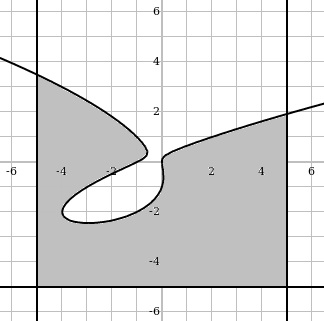
\includegraphics[width=0.5\linewidth]{aahw}
            \end{center}
  \question The following graph shows the acceleration of a rocket from launch until it reaches orbit. Given that the
            initial velocity of the rocket was \SI{0}{\foot\per\second}, find the final velocity of the rocket.
            \begin{center}
              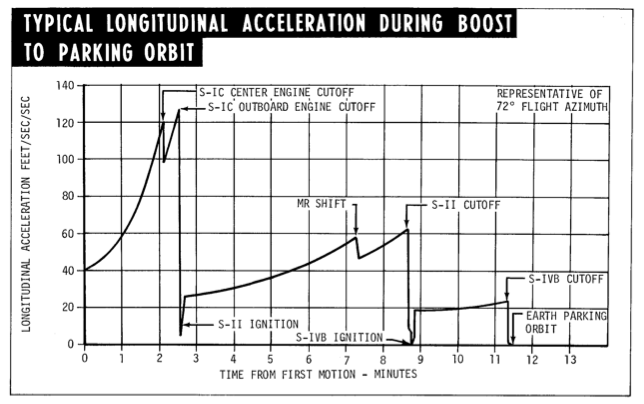
\includegraphics[width=0.7\linewidth]{acceleration-time}
            \end{center}
\end{questions}

\end{document}
